\chapter{语音情感识别的相关工作}
\label{cha:basic_konwledge}

\section{本章引论}
\label{sec:basic_konwledge_intro}
目前,语音情感识别方面的研究工作越来越多。由于情感感知的人为主观性比较强,这导致当前的研究不只是模型算法方面的研究,还包括心理学方面的研究和人文社会学方面的研究。此外,情感语音数据库的采集和标注也是一个很大的挑战。本章将对语音情感识别的相关工作进行简单的介绍,其中包括情感的定义、情感语音数据库、声学特征的抽取以及情感分类模型的构建四个方面。

\section{情感的定义}
\label{sec:emo_def}
情感在心理学上的定义为:“人对客观现实的一种特殊反映形式,是人对于客观事物是否符合人的需要而产生的态度的体验”~\cite{Van1983Recognition}。但这种定义太过宽泛,在实际的语音情感识别任务中无法运用,只有将情感通过数学量化表示后才能够被模型处理。目前对于情感的主流定义方式大致分为两种,分别是离散的情感类别标签定义和连续的情感维度空间定义,下面将分别对这两种定义进行介绍。

\subsection{离散的情感类别标签}
\label{ssec:discrete_label}
在我们的日常生活中,我们在描述自己的主观感受时,通常会用一些特定的词汇,例如高兴、愤怒、悲伤等等。在情感识别中通常会将这些词汇作为情感的类别,进而将任务转化为多分类问题。关于具体应该将情感分为那些类别,不同的学者有着不同的定义和划分,下面的表格\ref{tab:emo_categories}列举了不同的定义方式~\cite{Ortony1990What, Robinson2013Handbook}。

\begin{table}[htb]
  \centering
  \begin{minipage}[t]{0.8\linewidth} % 如果想在表格中使用脚注,minipage是个不错的办法
  \caption{不同学者对情感的定义~\cite{Ortony1990What, Robinson2013Handbook}}
  \label{tab:emo_categories}
    % \begin{tabular}{p{6cm}<{\centering} p{6cm}<{\centering}}
    \begin{tabularx}{\linewidth}{X<{\centering} X<{\centering}}
        \toprule[1.5pt]
        学者 & 情感类别 \\
        \midrule[1pt]
        Arnold & 愤怒,厌恶,无畏,忧郁,渴望,绝望,珍视,憎恨,希冀,爱慕,悲伤 \\
        Ekman, Friesen, Ellsworth & 愤怒,厌恶,恐惧,高兴,悲伤,惊讶 \\
        Fridja,Gray & 希冀,高兴,有趣,惊讶,渴望,悲伤 \\
        Izard & 愤怒,轻蔑,厌恶,悲伤,恐惧,内疚,有趣,高兴,羞愧,惊讶 \\
        James & 恐惧,悲伤,爱慕,愤怒 \\
        McDougall & 恐惧,厌恶,高兴,顺从,柔和的情感,渴望 \\
        Oatley, Johnson-Laird, Panksepp & 愤怒,厌恶,焦虑,高兴,悲伤 \\
        Plutchik & 认可,愤怒,希冀,厌恶,高兴,恐惧,悲伤,惊讶 \\
        Tomkins & 愤怒,有趣,轻蔑,厌恶,悲伤,恐惧,高兴,羞愧,惊讶 \\
        Watson & 恐惧,爱慕,愤怒 \\
        Weiner, Graham & 高兴,悲伤 \\
        \bottomrule[1.5pt]
    \end{tabularx}
  \end{minipage}
\end{table}

这种定义情感的方式的优点是简单、易懂,而且可以有比较明显的应用场景,这也使得当前关于情感识别的研究主要都是基于这种定义进行的,本文也主要是基于这种情感定义展开的。但缺点是对情感的描述能力有限,因为情感标签的描述太过模糊,对于一些复杂的情感无法准确的定义。例如,愤怒可以分为冷愤怒和热愤怒;又比如,高兴又可以分为不同的等级,从喜上眉梢,到眉飞色舞,再到手舞足蹈。

\subsection{连续的情感维度空间}
\label{ssec:continuous_space}
另外一种情感的定义方式是连续的情感维度空间定义~\cite{Cowie2002Emotion},这种定义将情感映射到一个笛卡尔空间坐标系中,不同的坐标轴分别代表不同的心理学属性,每一种情感都可以被视为坐标系中的一个点。常用的情感空间模型有激活度-效价(Activation-Valence)二维情感空间~\cite{Cowie2002Emotion}和激活度-效价-支配力(Activation-Valence-Dominance)三维情感空间~\cite{Cowie2002Emotion},下面的图\ref{fig:emo_space_2dim}和图\ref{fig:emo_space_3dim}分别是两种情感维度空间的示意图。

\begin{figure}[htb] % use float package if you want it here
    \centering
    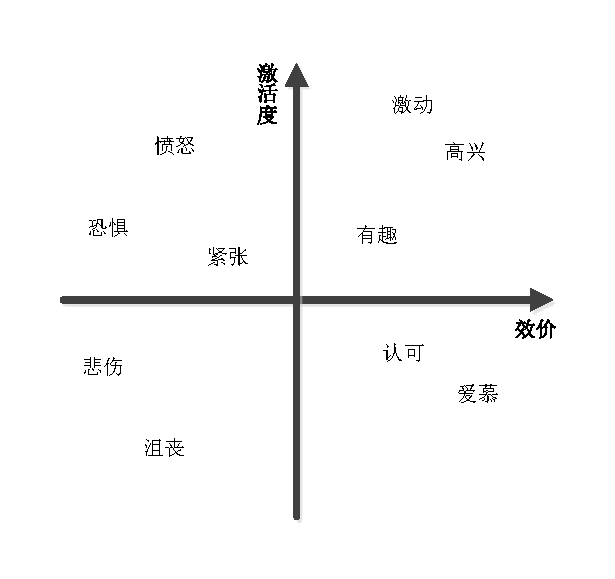
\includegraphics[height=10cm]{myfigures/emo_space_2dim}
    \caption{二维情感空间模型(激活度-效价)~\cite{Cowie2002Emotion}}
    \label{fig:emo_space_2dim}
\end{figure}

\begin{figure}[htb] % use float package if you want it here
    \centering
    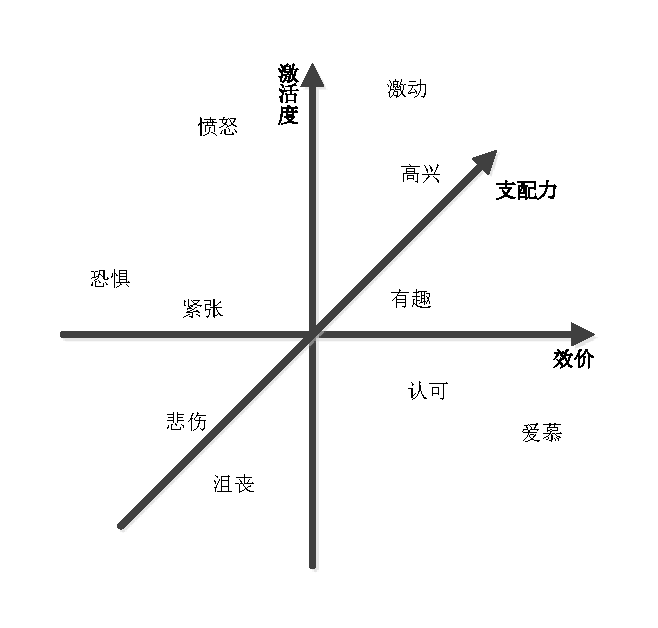
\includegraphics[height=10cm]{myfigures/emo_space_3dim}
    \caption{三维情感空间模型(激活度-效价-支配力)~\cite{Cowie2002Emotion}}
    \label{fig:emo_space_3dim}
\end{figure}

这种情感空间模型理论上可以描述任何情感,其中激活度代表情感的强烈程度,例如愤怒就是激活度非常高的情感。效价代表情感的积极性,例如悲伤就是一种积极性很低的情感,所以它的效价很低。支配力代表情感对别人的影响程度,例如高兴就是对别人影响比较大的一种情感,所以支配力比较大。情感空间模型将原先的标签分类问题转换为的对心理学属性值的回归问题,从而能够描述更为复杂的情感。但这种模型的的缺点是标记数据的成本太高,因为将主观情感量化为客观数值是一个繁重且难以保证质量的过程。

\section{情感语音数据库}
\label{sec:emo_speech_database}
在大多数的监督性机器学习问题中,训练数据一直是一个很大的问题,尤其是如何得到高质量的训练数据。对于语音情感识别而言,情感语音数据的获取和标注更是至关重要的问题。由于语音中情感信息的标注主要是要依靠人来完成的,但不同的人对情感的感知程度是不同的,所以同一句话有可能被不同的人标注为不同的情感。下面的两小节将主要介绍情感语音数据库的设计准则和一些常用的情感语音数据库。

\subsection{设计准则}
\label{ssec:design_criteria}
如何判断情感语音数据库能够模拟真实的应用场景,这需要相应设计准则来指导,下面将介绍几种主要的设计准则。

自然语音还是表演式语音?通常来说,最符合实际的语音数据应该是从日常生活的对话中收集~\cite{Campbell2000Databases},例如广播电台,电话客服系统等,这样的录音包含有最自然的情感表达。但不幸的是,由于一些法律和道德的原因,这样的数据被禁止用作研究目的。所以现在大多数情感语音数据库都采用了另一种替代方式,聘请一些专业的演员在录音室中去演绎预定的情感语音~\cite{Mazuka2015Emotions}。尽管有一些学者认为这样得到的语音情感表现过于夸张,和实际的自然语音不一致,但是这并不影响用这种数据库来探索声学表现和情感之间的相关性。

录制时如何唤醒情感?在录制情感语音数据库时,首先需要做的就是唤醒说话人的情感,通常有三种唤醒方式。第一种就是让说话人根据规定情感进行表演~\cite{Lee2005Toward},但这种方式得到情感表现过于夸张,和自然语音中的表现不一致。第二种就是将说话人置于某些特定的环境下来激起对特定的情感反应~\cite{Batliner2000Desperately},例如通过一些诱发式的交谈,或者一些交互式的游戏。第三种就是让标注者从生活中录制的自然语音去标注出有情感的句子~\cite{Johnstone2005Affective},这种语音最为真实,但是标注成本太高,需要大量的人力劳动。

不同情感的数据量是否平衡?由于在日常生活中,不同的情感触发的几率并不相同,所以会导致包含不同情感的语音数量也不同,例如中性语音是日常生活中出现最多的。这种分布不平衡的数据库会导致在训练分类器时出现偏置,使得分类器更趋向于预测为数据量多的那种情感。有一些数据库为了保持分布平衡会保证不同情感的句子数量基本一致~\cite{Burkhardt2005A}。但一些研究者~\cite{Hansen1997Getting, Morrison2007Ensemble}认为这种分布正体现了实际应用场景的情感出现概率,所以应该通过调整模型来包含这种信息。

情感语音是否应该保证说话人以及说话内容无关?由于不同的人表达情感的方式不相同,如果数据库中只包含个别人的语音就会导致模型不够强健,无法识别其他人的语音。应该保证尽可能多的说话人。还有就是语音中的语言学信息通常和情感都是强相关的,在录制数据库时是否应该排除掉语言学信息的影响,也是需要关注的问题。现在大多数研究者的观点是对于提前准备台词的表演型数据库,由于情感触发和文本是相关联的,所以并不适合用于语音情感识别。

\subsection{常用的情感语音数据库}
\label{ssec:available_database}
由于大多数的情感语音数据库都不是公开的,所以只有很少的基准数据库可以被研究者们共享。但由于情感语音数据的录制没有标准的规范,所以导致不同数据库的录制方式各不相同,下面的表格列举了一些常用的情感语音数据库。

\begin{table}[htb]
\centering
    \begin{minipage}[t]{1.0\linewidth} % 如果想在表格中使用脚注,minipage是个不错的办法
    \caption{常用的情感语音数据库}
    \label{tab:emo_database}
        % \begin{tabular}{p{6cm}<{\centering} p{6cm}<{\centering}}
        \begin{tabularx}{\linewidth}{X<{\centering} X<{\centering} X<{\centering} X<{\centering}}
            \toprule[1.5pt]
            数据库名 & 语言 & 大小 & 来源 \\
            \midrule[1pt]
            LDC~\cite{LibermanEmotional} & 英语 & 7人$\times$15种情感$\times$10个句子 & 专业演员 \\
            柏林情感语音数据库~\cite{Burkhardt2005A} & 德语 & 10人$\times$7种情感$\times$10个句子 & 专业演员 \\
            丹麦情感语音数据库~\cite{Engberg1997Design} & 丹麦语 & 4人$\times$5种情感 & 非专业演员 \\
            Natural~\cite{Morrison2007Ensemble} & 普通话 & 11人$\times$2种情感 & 呼叫中心 \\
            ESMBS~\cite{Nogueiras2012Speech} & 普通话 & 12人$\times$6种情感 & 非专业演员 \\
            INTERFACE~\cite{Hozjan2002Interface} & 英语,斯洛文尼亚语,西班牙语,法语 & 635个句子 & 专业演员 \\
            KISMET~\cite{Breazeal2002Recognition} & 美式英语 & 3人$\times$5种情感 & 非专业演员 \\
            BabyEars~\cite{Slaney2003Baby} & 英语 & 12人$\times$3种情感 & 父亲和母亲 \\
            SUSAS~\cite{Hansen1997Getting} & 英语 & 16000个句子 & 压力下的模仿 \\
            MPEG-4~\cite{Schuller2005Speaker} & 英语 & 2440个句子 & 美国电影 \\
            北航情感语音数据库~\cite{Fu2008Speaker} & 普通话 & 7人$\times$5种情感$\times$20个句子 & 非专业演员 \\
            FERMUS \uppercase\expandafter{\romannumeral3}~\cite{Schuller2002Towards} & 德话,英语 & 13人$\times$7种情感 & 诱发环境 \\
            KES~\cite{Kim2007Speech} & 韩语 & 5400个句子 & 非专业演员 \\
            CLDC~\cite{Zhou2006Speech} & 汉语 & 1200个句子 & 非专业演员 \\
            Pereira~\cite{Pereira2000Dimensions} & 英话 & 2人$\times$5种情感$\times$8个句子 & 非专业演员 \\
            IEMODB~\cite{Busso2008IEMOCAP} & 英话 & 10人$\times$9种情感 & 专业演员 \\
            \bottomrule[1.5pt]
        \end{tabularx}
    \end{minipage}
\end{table}

% \uppercase\expandafter{\romannumeral3}

这里主要介绍下IEMODB~\cite{Busso2008IEMOCAP}这个情感语音数据库,因为本文的研究工作主要是以这个数据库作为实验基础的。IEMODB主要被设计用于多模态情感表现研究,它包括肢体动作、音频和视频,一共有5个部分,每个部分包括10个主题,总共有接近12个小时的数据。每一个部分包含一个不同的对话场景,会有一个男演员和一个女演员分别表演规定好的剧本,以及在一个对话中诱发情感。至少三个标记员对同一句话标记情感类别,包括高兴、悲伤、中性、愤怒、惊讶、激动、沮丧、厌恶、恐惧这些情感标签。这个数据库被许多的研究工作采用,因此可以用来与其他研究工作的实验结果作对比。

\section{声学特征的抽取}
\label{sec:acoustic_feature_extract}
语音情感识别中一个重要的问题就是抽取与情感相关的声学特征,因为这些特征作为模型的输入会直接影响到最终的分类效果。下面将会对特征的选择和抽取方式做出介绍。

\subsection{人工选择情感相关的声学特征}
\label{ssec:artifical_select}
在大多数研究中,声学特征都是通过以往的一些经验选择或者设计出来的。用于语音情感识别的声学特征大致可以分为三类,分别为韵律学相关的特征、  谱相关的特征以及声音质量相关的特征,如图\ref{fig:acoustic_feature_type}所示。

\begin{figure}[htb] % use float package if you want it here
    \centering
    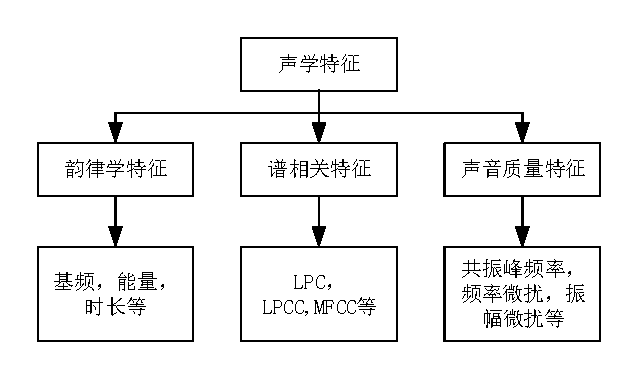
\includegraphics[height=10cm]{myfigures/acoustic_feature_type}
    \caption{不同类型的声学特征}
    \label{fig:acoustic_feature_type}
\end{figure}

韵律是指人说话时的节奏、轻重、快慢和音高等方面的的变化,它与语音中携带的语言学信息并没有太大的关联,但却决定着一句话给听众的感觉,因此又被称为“超音段特征”或“辅助语言学特征”。这种韵律学相关的特征被广泛的应用在语音情感识别领域,主要包括基频、时长、能量等。根据Williams和Stevens的研究~\cite{Williams1981Vocal},语音情感的激活度会显著的影响频谱上的能量分布、基频的大小以及停顿的时长,其他一些研究~\cite{Johnstone2000Vocal, Cowie2003Describing}也证明了这一结论。此外,有研究证明这些特征也和基本情感类别有着很强的关联,例如Murray和Arnott的研究~\cite{Murray1993Toward}证明快的说话速率与愤怒是相关联的,但也有些研究~\cite{Ackroyd1997Digital, Cahn1990The}表明部分情感的韵律学比较相似,例如愤怒、恐惧、高兴和惊讶都有相似的基频。

谱相关的特征被认为与声道对语音信号的调制相关联,这类特征之前一直被语音识别广泛的应用,但现在一些研究证明这类特征在情感识别中也发挥很大的作用,例如线性预测系数(Linear Prediction Coefficients, LPC)~\cite{Ackroyd1997Digital},线性预测倒谱系数(Linear Prediction Cepstral Coefficients, LPCC)~\cite{Atal1974Effectiveness}以及梅尔频率倒谱系数(Mel-frequency Cepstral Coefficients, MFCC)~\cite{Rabiner1999Fundamentals, Proakis1993Discrete}。Nwe等人~\cite{Nogueiras2012Speech}发现语音信号不同频段的能量分布和情感类别有着相关性,例如高兴的语音通常在高频段有着较高的能量,而悲伤的语音在高频段的能量却相对较低。

声音质量特征是人对声音的一种主观评价,主要用于衡量声音的流利和清晰程度。当人在情绪比较激动的时候,通常会出现哽咽、颤音、喘息之类的反应,这会导致声音质量发生变化。因此,研究者~\cite{Gobl2003The}认为声音质量特征也可以反映情感的变化。声音质量特征包括共振峰频率及其带宽、频率微扰、振幅微扰、声门参数等。Lugger等人~\cite{Lugger2007The, Lugger2008Psychological, Lugger2015Combining}通过使用共振峰频率和带宽作为特征取得了很不错的效果。Li等人~\cite{Li2007Stress}也采用梅尔频率倒谱系数加频率微扰和振幅微扰,取得超过只使用梅尔频率倒谱系数的效果。

\subsection{特征选择算法筛选情感相关的声学特征}
\label{ssec:algorithm_select}
声学特征有许多种,选择与情感相关的特征除了依靠人工挑选以外,还可以通过一些特征选择算法来自动选出相关的特征。假设我们有一个很大的特征集合,特征选择算法所要做的就是规定一种指标,例如熵增益~\cite{Dhillon2003A}或者识别准确率~\cite{Dietterich1998Approximate},然后通过特征的各种组合来选取出那些指标最好的特征子集。这样既可以减少输入特征的数量,降低计算量,又可以去除无效特征的干扰,大致流程如图\ref{fig:feature_select_flow}所示。

\begin{figure}[htb] % use float package if you want it here
    \centering
    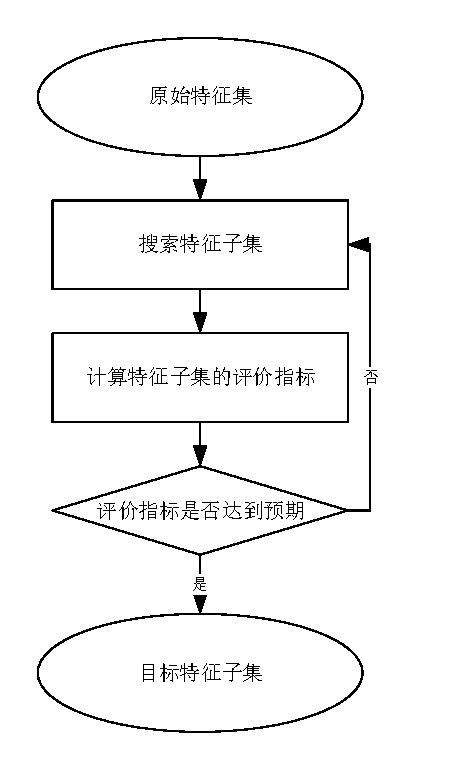
\includegraphics[height=10cm]{myfigures/feature_select_flow}
    \caption{特征选择流程图}
    \label{fig:feature_select_flow}
\end{figure}

特征选择算法有许多,例如序列浮动前向选择算法(Sequential Floating Forward Selection, SFFS)~\cite{Ververidis2008Fast}通过迭代的方法选择出接近最优的特征子集;还有遗传算法(Genetic Algorithm, GA)~\cite{Yang1998Feature}是一种模拟生物进化的算法,它通过不断地繁殖和变异来筛选出最优的特征子集。除了特征选择算法以外,还有一些特征空间转换的算法也可以降低输入特征的维度,例如主成分分析(Principal Component Analysis, PCA)~\cite{Ben2003Detecting}和线性判别分析(Linear Discriminant Analysis, LDA)~\cite{Blum1997Selection},它们可以通过矩阵运算将高维特征向量转换到低维特征向量,从而减少计算量。


\subsection{深度神经网络抽取情感相关的声学特征}
\label{ssec:dnn_extract}
在近几年,深度学习方法和工具被引入到语音信号处理领域~\cite{Han2014Speech, Lee2015High, Huang2014Speech, Le2013Emotion, Rana2016Emotion, Chernykh2017Emotion},研究者发现采用深度神经网络从原始语音信号来提取特征,可以取得比人工定义的声学特征更好的结果,同时这也衍生出了端到端语音情感识别系统。现在有很多的神经网络结构都被用于特征抽取,例如最早的工作是Jaitly等人~\cite{Jaitly2011Learning}通过受限玻尔兹曼机(Restricted Boltzmann Machine, RBM)从原始语音信号上得到一种有利于语音识别的中间表示。Bhargava等人~\cite{Bhargava2015Architectures}则是通过堆叠的全连接神经网络从原始语音信号得到瓶颈特征,并且取得了和使用梅尔频率倒谱系数(Mel-frequency Cepstral Coefficients, MFCC)相近的效果。George等人~\cite{Trigeorgis2016Adieu}提出一种使用卷积神经网络(Convolution Neural Network, CNN)从原始语音信号提取特征,然后通过长短时记忆循环神经网络(Long-Short Term Memory Recurrent Neural Network, LSTM-RNN)捕获输入序列的时序信息并最终输出不同情感的后验概率,并且他们发现长短时记忆循环神经网络(Long-Short Term Memory Recurrent Neural Network, LSTM-RNN)不同节点的输出和一些声学特征有很强的相关性。Satt等人~\cite{Satt2017Efficient}也采用了相似的神经网络结构,但不同的是他们从语谱图上抽取特征而非原始语音信号。他们认为在语谱图上可以更方便的进行去噪的操作,并且他们在公开情感语音数据集IEMOCAP上取得了超过之前最好结果(state-of-the-art)的准确率。

\section{情感分类模型的构建}
\label{sec:emotion_cls}

在抽取声学特征之后,需要构建分类模型来判别特征向量所属的情感类别。事实上,目前情感语音识别的大多数研究都是关注在这一步骤上,下面我们将介绍情感分类模型的相关的技术,主要包括传统的分类模型和深度学习的分类模型。

\subsection{基于传统机器学习的情感分类模型}
\label{ssec:traditional_cls}

许多传统机器学习中的分类算法已经被运用在语音情感识别任务上,例如隐马尔可夫模型(Hidden Markov Model, HMM),高斯混合模型(Gaussian Mixture Models, GMM),支持向量机(Support Vector Machine, SVM)等。目前并没有公认的最适合语音情感识别的分类器,每一种分类器都有各自的优缺点,下面我们将分别介绍几种常用的分类器模型。

HMM被广泛地应用在语音识别领域,例如孤立词的识别和端点检测。这是因为它和语音信号的产生机制十分相似~\cite{Rabiner2007An}。HMM是一个包含一阶马尔科夫链的双随机过程,分别包含隐藏的转移状态和可观测的输出,其中隐藏状态是用来建模语音信号的时序信息。在数学上,为了通过HMM给一个可观测序列$\mathbf{x}_1,...,\mathbf{x}_T$建模,我们假设一个马尔科夫链可以用于生成观测序列,让$K$代表状态的数量,$\pi_i, i=1,...,K$代表不同状态的初始概率,$a_{ij}, i=1,...K, j=1,...,K$代表从状态$i$到状态$j$的转移概率。通常HMM的参数都是通过最大似然的方法来估计。假设实际的状态序列是$s_1,...,s_T$,观测序列的似然度可以通过下面的公式给出:
\begin{equation}
\label{equ:output_pro}
    \begin{aligned}
        p(\mathbf{x}_1,s_1,...,\mathbf{x}_T,s_T) &= \pi_{s_1}b_{s_1}(\mathbf{x}_1)a_{s_1,s_2}b_{s_2}(\mathbf{x}_2)...a_{s_{T-1},s_T}b_{s_T}(\mathbf{x}_T) \\
        &= \pi_{s_1}b_{s_1}(\mathbf{x}_1)\prod\limits_{t=2}^Ta_{s_{t-1},s_t}b_{s_t}(\mathbf{x}_t)
    \end{aligned}
\end{equation}
其中,$b_i(\mathbf{x}_t) \equiv P(\mathbf{x}_t|s_t = i)$是第$i$个状态的输出概率。它既可以是离散的概率分布,也可以是连续的概率密度。因为真实的状态序列并不知道,所以在给定输出序列时,我们必须对所有可能的状态序列的似然度求和,如下面的公式:
\begin{equation}
\label{equ:output_pro_sum}
        p(\mathbf{x}_1,...,\mathbf{x}_T) = \sum\limits_{s_1,...,s_T}\pi_{s_1}b_{s_1}(\mathbf{x}_1)\prod\limits_{t=2}^Ta_{s_{t-1},s_t}b_{s_t}(\mathbf{x}_t)
\end{equation}
幸运的是,一种计算似然度的高效算法已经提出,可以将时间复杂度降低至$O(KT)$。在训练阶段,HMM的参数通过最大化公式\ref{equ:output_pro_sum}的似然度来获得,这通常可以使用期望最大化(Expectation Maximization, EM)算法~\cite{Dempster1977Maximum}来实现。在语音识别中,HMM的结构通常是从左到右的,因为这种结构符合语音信号的时序特性。但在语音情感识别中,除了使用从左到右结构以外,全连接的结构也会被使用,因为情感信息可能只集中在某一个小的时间段内,而不是所有的时间段都是均匀的。HMM已经被许多语音情感识别的研究所采用, 在Nwe的工作~\cite{Nogueiras2012Speech}中,一个基于HMM的语音情感识别系统用于区分6种基本情感,模型为不同的情感和不同的说话人分别构建了一个四状态的全连接HMM。在Lee的工作~\cite{Lee2004Emotion}中,两个不同的HMM模型被提出,一种是普通的HMM加GMM的模型,另一种则是和语音识别一样先构建对音素的HMM模型,然后构建音素序列到情感类别的映射模型,作者表示采用对音素建模的方式比普通的方式可以取得更好的效果。

GMM是一种采用多个高斯分布变量的概率模型,它可以被考虑为一种只包含一个状态的HMM~\cite{Vlassis2002A, Reynolds1995Robust}。GMM的训练和测试过程相比于一般的连续HMM更为简单,这也使得它被广泛的使用在语音情感识别中,但是GMM无法建模语音信号的时序信息。在GMM模型构建中最困难的就是决定需要多少个高斯分量,最简单的方法就是人工尝试设置不同的数量,然后看模型的效果。此外,期望最大化算法可以被用来自动调整高斯分量的数量和模型的参数。GMM相关的工作也有许多,在Breazeal的工作~\cite{Breazeal2002Recognition}中,一个GMM分类器被用在KISMET情感语音数据库上,获得了77.87\%的平均准确率,后面又采用分层决策的策略取得了81.94\%的平均准确率。GMM也被用在其他的情感语音数据库中,例如BabyEars情感语音数据库~\cite{Slaney2003Baby},模型尝试了1-100的高斯分量数量,最终在数量为10的时候取得了最好的结果,达到平均准确率为75\%。在FERMUS \uppercase\expandafter{\romannumeral3}数据库上也获得相似的结果,16个分量的GMM被用来为每种情感建模,平均准确率达到了74.83\%。

SVM是一种非常流行的分类算法~\cite{Burges2008A},它在许多的模式识别任务中均取得了很不错的效果。SVM模型主要是利用核函数将在低维特征空间线性不可分的向量映射到高维空间,使得数据可以被线性分类器划分。相比于HMM和GMM,SVM可以得到全局最优的分类边界~\cite{Burges1998A},但是对于不可分的数据,它又不得不采用一些启发式的方法。事实上,并没有系统性的方法可以用来选择核函数,因此,转换后的数据可分性是无法保证的。在大多数模式识别任务,包括语音情感识别,并不建议找到训练数据的最佳分类面,因为这可能会导致过拟合。有许多语音情感识别的研究都在使用SVM~\cite{Lee2004Emotion, Schuller2004Speech, Kwon2003Emotion, Pierre2003The},它们都取得了相似的结果。其中一个工作将SVM通过三种不同的策略从二分类器转换为多分类器。第一种策略是将多分类任务转换为多个二分类任务,每个二分类任务将一个情感看作一类,其他所有情感看作一类,所有二分类器的结果中输出最大的情感类别代表最终的识别结果。第二种策略是将所有二分类器的输出传递给一个三层感知机,让它完成最后的决策。第三种方法是采用分层决策的策略,在不同的阶段决策不同的情感。这三种模型在FERMUS \uppercase\expandafter{\romannumeral3}数据库上做测试,分别得到了76.12\%,75.45\%和81.29\%的分类准确率。

除了采用单一的分类模型以外,多分类器混合模型也被用于语音情感识别。有三种不同的方法来组合不同的分类器~\cite{Kuncheva2004Combining, Lugger2015Combining}。第一种是分层判决的方法,每个分类器都被放置在一棵决策树的各个节点,输入从根节点出发,不断向下探索,最终到达叶子节点时会被划分到唯一的情感类别。在Lugger的工作~\cite{Lugger2008Psychological}中,分层的模型在柏林情感语音数据库中测试,其中采用了考虑心理学情感属性的二阶段和三阶段分层分类系统。二阶段的方法可以达到83.5\%的分类准确率,三阶段的方法可以达到88.8\%的分类准确率。第二种是顺序串行的判决方法,就是依次采用不同的分类器对数据进行分类,当前的分类器会影响下一个分类器的结果。第三种是多分类器并行的判决方法,就是同时训练多个分类器,然后将所有分类器的结果进行决策融合得到最终的分类结果。

\subsection{基于深度学习的情感分类模型}
\label{ssec:dnn_cls}

近几年来,深度学习的模型开始变的越来越流行,这种方法也在语音情感识别中也取得了很不错的效果。相比于传统的机器学习模型,深度学习模型可以对更复杂的非线性映射关系进行建模。已经有许多的深度神经网络结构被提出,例如自编码神经网络(Auto-Encode Neural Network),卷积神经网络(Convolution Neural Network, CNN),循环神经网络(Memory Recurrent Neural Network, RNN),受限玻尔兹曼机(Restricted Boltzmann Machine, RBM)等。其中一部分工作仍然是采用传统的声学特征来进行建模,但近几年也开始出现直接基于原始信号的端到端的语音情感识别。

基于传统声学特征的深度学习分类模型已经有很多工作,Han等人~\cite{Han2014Speech}采用普通的深度神经网络(Deep Neural Network, DNN)得到不同的语音子段在不同情感上的概率分布,然后通过统计学方法的方法将所有子段的概率分布融合得到整个句子的特征表示,最后采用一种单层的神经网络结构,叫做极限学习器(Extreme Learning Machine, ELM)来得到最终的情感类别。在IEMOCAP数据库~\cite{Busso2008IEMOCAP}上,这种方法取得了48.2\%的不加权准确率(Unweighted Accuracy, UA)和54.3\%的加权准确率(Weighted Accuracy, WA)。Kim等人~\cite{Kim2013Deep}提出采用深度信念网络(Deep Belief Network, DBN)代替传统的特征选择算法,来获得更为有效的特征表示。 DBN是由多层RBM堆叠而成,可以采用无监督的方式训练,在IEMOCAP数据库~\cite{Busso2008IEMOCAP}上取得了66.12\%的不加权准确率。Deng等人~\cite{Deng2013Sparse}采用一种自编码神经网路来进行特征的转换学习,他们先通过大量未标记的情感语音训练自编码神经网络,从而可以找到更为有效的特征表示,然后再用标记数据对自编码神经网络进行微调,在5个不同的情感语音数据库上进行交叉测试均取得了不错的效果。

基于原始信号的端到端的分类模型也开始有一些工作被提出。George等人~\cite{Trigeorgis2016Adieu}提出使用CNN从原始语音信号提取特征,然后通过LSTM-RNN捕获输入序列的时序信息并最终输出不同情感的后验概率。作者认为通过CNN和RNN可以将时序信息编码到特征表示中,并且他们发现LSTM-RNN不同节点的输出和一些传统的声学特征有很强的相关性。实验结果表明这种端到端的方式可以取得比传统声学特征更好的效果。Satt等人~\cite{Satt2017Efficient}也采用了相似的神经网络结构,但不同的是他们从语谱图上抽取特征而非原始语音信号。他们认为在语谱图上可以更方便的进行去噪的操作,并且他们在公开情感语音数据集IEMOCAP~\cite{Busso2008IEMOCAP}上取得了超过之前最好结果(The State of Art)的准确率。

\section{本章小结}
\label{sec:basic_konwledge_summary}

本章简单介绍了语音情感识别相关的研究工作,包括情感的定义、情感语音数据库、情感相关的声学特征和一些常用的情感分类模型。这些工作包含了当前语音情感识别领域的主要关注点,为后面介绍自己的研究工作提供了铺垫。

% \chapter{中华人民共和国}
% \label{cha:china}

% \section{其它例子}
% \label{sec:other}

% 在第~\ref{cha:intro} 章中我们学习了贝叶斯公式~(\ref{equ:chap1:bayes}),这里我们复
% 习一下:
% \begin{equation}
% \label{equ:chap2:bayes}
% p(y|\mathbf{x}) = \frac{p(\mathbf{x},y)}{p(\mathbf{x})}=
% \frac{p(\mathbf{x}|y)p(y)}{p(\mathbf{x})}
% \end{equation}

% \subsection{绘图}
% \label{sec:draw}

% 本模板不再预先装载任何绘图包(如 \pkg{pstricks,pgf} 等),完全由用户来决定。
% 个人觉得 \pkg{pgf} 不错,不依赖于 Postscript。此外还有很多针对 \LaTeX{} 的
%  GUI 作图工具,如 XFig(jFig), WinFig, Tpx, Ipe, Dia, Inkscape, LaTeXPiX,
% jPicEdt, jaxdraw 等等。

% \subsection{插图}
% \label{sec:graphs}

% 强烈推荐《\LaTeXe\ 插图指南》!关于子图形的使用细节请参看 \pkg{subcaption} 宏包的说明文档。

% \subsubsection{一个图形}
% \label{sec:onefig}
% 一般图形都是处在浮动环境中。之所以称为浮动是指最终排版效果图形的位置不一定与源文
% 件中的位置对应\footnote{This is not a bug, but a feature of \LaTeX!},这也是刚使
% 用 \LaTeX{} 同学可能遇到的问题。如果要强制固定浮动图形的位置,请使用 \pkg{float} 宏包,
% 它提供了 \texttt{[H]} 参数,比如图~\ref{fig:xfig1}。
% \begin{figure}[H] % use float package if you want it here
%   \centering
%   
\includegraphics{thu-whole-logo}
%   \caption{利用 Xfig 制图}
%   \label{fig:xfig1}
% \end{figure}

% 大学之道,在明明德,在亲民,在止于至善。知止而后有定;定而后能静;静而后能安;安
% 而后能虑;虑而后能得。物有本末,事有终始。知所先后,则近道矣。古之欲明明德于天
% 下者,先治其国;欲治其国者,先齐其家;欲齐其家者,先修其身;欲修其身者,先正其心;
% 欲正其心者,先诚其意;欲诚其意者,先致其知;致知在格物。物格而后知至;知至而后
% 意诚;意诚而后心正;心正而后身 修;身修而后家齐;家齐而后国治;国治而后天下
% 平。自天子以至于庶人,壹是皆以修身为本。其本乱而未治者 否矣。其所厚者薄,而其所
% 薄者厚,未之有也!

% \hfill —— 《大学》


% \subsubsection{多个图形}
% \label{sec:multifig}

% 如果多个图形相互独立,并不共用一个图形计数器,那么
% 用 \texttt{minipage} 或者\texttt{parbox} 就可以。否则,请参看
% 图~\ref{fig:big1-subcaptionbox},它包含两个小图,分别是图~\ref{fig:subfig1}和
% 图~\ref{fig:subfig2}。推荐使用 \cs{subcaptionbox},因为可以像
% 图~\ref{fig:big1-subcaptionbox} 那样对齐子图的标题,也可以使用 \pkg{subcaption}
% 宏包的 \cs{subcaption}(放在 minipage中,用法同\cs{caption})或
% 是 \pkg{subfigure} 、\pkg{subtable}环境,像图~\ref{fig:big1-subfigure},不要再
% 用 \cs{subfloat}、\cs{subfigure} 和 \cs{subtable}。

% \begin{figure}[h]
%   \centering%
%   \subcaptionbox{第一个小图形\label{fig:subfig1}}[3cm] %标题的长度,超过则会换行,如下一个小图。
%     {
\includegraphics[height=3cm]{thu-fig-logo}}%
%   \hspace{4em}%
%   \subcaptionbox{第二个小图形,注意这个图略矮些。如果标题很长的话,它会自动换行\label{fig:subfig2}}
%       {
\includegraphics[height=2cm]{thu-text-logo}}
%   \caption{包含子图形的大图形(subcaptionbox示例)}
%   \label{fig:big1-subcaptionbox}
% \end{figure}
% \begin{figure}[h]
%   \centering%
%   \begin{subfigure}{3cm}
%     
\includegraphics[height=3cm]{thu-fig-logo}
%     \caption{第一个小图形}
%   \end{subfigure}%
%   \hspace{4em}%
%   \begin{subfigure}{0.5\textwidth}
%     
\includegraphics[height=2cm]{thu-text-logo}
%     \caption{第二个小图形,注意这个图略矮些。subfigure中同一行的子图在顶端对齐。}
%   \end{subfigure}
%   \caption{包含子图形的大图形(subfigure示例)}
%   \label{fig:big1-subfigure}
% \end{figure}

% 古之学者必有师。师者,所以传道受业解惑也。人非生而知之者,孰能无惑?惑而不从师,
% 其为惑也,终不解矣。生乎吾前,其闻道也固先乎吾,吾从而师之;生乎吾後,其闻道也亦
% 先乎吾,吾从而师之。吾师道也,夫庸知其年之先後生於吾乎!是故无贵无贱无长无少,道
% 之所存,师之所存也。

% 嗟乎!师道之不传也久矣,欲人之无惑也难矣。古之圣人,其出人也远矣,犹且从师而问焉;
% 今之众人,其下圣人也亦远矣,而耻学於师。是故圣益圣,愚益愚。圣人之所以为圣,愚
% 人之所以为愚,其皆出於此乎?爱其子,择师而教之,於其身也,则耻师焉,惑焉。彼童子
% 之师,授之书而习其句读者,非吾所谓传其道、解其惑者也。句读之不知,惑之不解,或师
% 焉,或不焉,小学而大遗,吾未见其明也。巫医、乐师、百工之人不耻相师,  士大夫之族
% 曰“师”曰“弟子”之云者,则群聚而笑之。问之,则曰:彼与彼年相若也,道相似也,位
% 卑则足羞,官盛则近谀。呜呼!师道之不复,可知矣。巫医、乐师、百工之人。吾子不齿,
% 今其智乃反不能及,其可怪也欤!圣人无常师。孔子师郯子、苌子、师襄、老聃。郯子之徒,
% 其贤不及孔子。孔子曰:“三人行,必有我师。”是故弟子不必不如师,师不必贤於弟子。
% 闻道有先後,术业有专攻,如是而已。

% 如果要把编号的两个图形并排,那么小页就非常有用了:
% \begin{figure}
% \begin{minipage}{0.48\textwidth}
%   \centering
%   
\includegraphics[height=2cm]{thu-whole-logo}
%   \caption{并排第一个图}
%   \label{fig:parallel1}
% \end{minipage}\hfill
% \begin{minipage}{0.48\textwidth}
%   \centering
%   
\includegraphics[height=2cm]{thu-whole-logo}
%   \caption{并排第二个图}
%   \label{fig:parallel2}
% \end{minipage}
% \end{figure}

% 李氏子蟠,年十七,好古文、六艺,经传皆通习之,不拘於时,学於余。余嘉其能行古
% 道,作师说以贻之。

% \hfill —— 韩愈(唐)
